\documentclass{article}
\usepackage{graphicx}
\begin{document}

\title{SNEWS Operational Mode 1.0}         
\date{Effective \today}
\maketitle

This document provides specifications for the instance of
the class defined in the SNEWS Operational Mode Template document.


\section{Participating Experiments}

The participating experiments for this mode are:

\begin{itemize}
\item Super-K,
\item LVD,
\item SNO.
\end{itemize}

\section{Privacy Agreement}\label{privacy}

The SNEWS inter-experiment privacy agreement can be found at \\
{\tt http://cyclo.mit.edu/snnet/privacy/}.

\section{Client Computer Management}

Criteria of the privacy agreement (section~\ref{privacy}) regarding
access to SNEWS-related accounts on the client computer should be
strictly observed. In addition, the following are recommended:

\begin{itemize}
\item Outside the main domain of the 
client computer, TCP/IP access to the client machine should be restricted.
\item Login to the client computer should permitted only to SNEWS subgroup 
members.
\item The TCP/IP address of the client computer should be known only to 
SNEWS subgroup members.
\end{itemize}

\section{Server Computer Management}

There is one server machine located at Brookhaven
National Laboratory, and the BNL SNEWS sysadmin is Brett Viren.
The details of the server management, which address all
security and maintenance issues, can be found
in the Memorandum of Understanding at\\
{\tt http://cyclo.mit.edu/snnet/bnl\_mou/}.

\section{Client-Server Communications}\label{alarm}
\begin{itemize}

\item Each participating experiment may generate and send to the server
different types of alarm datagrams.
The alarm datagrams include a packet type, and a level flag.
The packet type can be PING, ALARM, or RETRACTION.
The level flag can be TEST, GOOD, POSSIBLE, RETRACTED or OVERRIDE.  
Datagrams having packet field values which do not 
belong to any of these categories are discarded by the server.

\noindent \underline{Packet Types}

\begin{itemize}
\item PING: Ping packets are used for test purposes only
and cause nothing more than a message printed to the coincidence
server log.

\item ALARM: Alarm packets contain information about individual
experiment alarms; what the server does with them depends on the
level flag.

\item RETRACTION:  Retraction packets contain information about
previously sent alarms to be retracted from the server's alarm queues.

\end{itemize}

\noindent \underline{Level Flags}

\begin{itemize}

\item TEST: This flag indicates a datagram packet intended for test use
as well as for any high-rate test mode.  The alarm level
is set to {\it 0}.

\item POSSIBLE : This flag indicates an alarm
generated during scheduled operations (i.e. maintenance, calibration,
tests, etc.) or other known anomalous conditions. It is up to each
experiment to set this flag inside the packet when appropriate.  The
alarm level is set to {\it 1}.

\item GOOD: This flag indicates an alarm generated during
normal detection conditions.  The alarm level is set to {\it 2}.

\item RETRACTED: This flag is set for retraction 
packets (note that this information is redundant -- all packets of
RETRACTION type will be retracted regardless of level flag).  The
alarm level is set to {\it -1}.

\item OVERRIDE: This flag indicates an alarm 
that has been confirmed as good.  The alarm level is set to {\it 3}.

\end{itemize}
 
\item The details of the SNEWS datagram structure should
not be propagated beyond the SNEWS subgroup.

\item The client datagrams employ TCP protocol and 
are encrypted using OpenSSL.  
The server process listens for connections on a specified port,
and when a client initiates a connection, it employs several layers
of checks to validate the origin of the datagram:
\begin{enumerate}
\item The server process employs a {\tt tcp\_wrappers hosts\_access}
call to check the IP of the client machine against the lists in
{\tt hosts.allow/deny}.  These lists allow only the IP addresses
of the client machines of the involved experiments to submit packets.
\item
The client and server exchange certificates which have been
verified by the SNEWS Certificate Authority, and reject
connections if the check fails.
\item There is an additional check of specific client machine
IP addresses against a list of allowed addresses before data is exchanged.
\end{enumerate}
\end{itemize}

\section{SNEWS Shift}

SNEWS shifts will be coordinated by Kate Scholberg, and will be run on
a week by week basis.    SNEWS shifters must be subgroup members.
The shifter must have cellular communications capability, and
have quick access to a computer during the 24 hour period of
his or her shift.


\subsection{Shift Alert Responsibilities}

Upon receipt of any coincidence message, either SILVER or GOLD, the
shifter must immediately log on to the server computer to check that
SNEWS code is running correctly, according to logs.  If everything
is in order, he or she must follow
the alert procedures outlined in sections \ref{SILVER}-\ref{GOLD}.  If
something seems to be wrong, the shiftworker must contact the
relevant people.

\subsection{Shift Maintenance and Monitoring Responsibilities}

The shifter has in addition some daily monitoring responsibilities.
The online shift checklist is available at\\
\texttt{https://cyclo.mit.edu/snnet/wg/shift/}.
Twice per 24 hour period (morning and evening), 
the shifter must check the following:

\begin{itemize}
\item The gcserver process is running normally.
\item The server log output seems normal.
\item The shifter's cellular communications capability is active,
batteries charged, etc.

\end{itemize}

The shifter must make an entry in the online logbook and record any
anomalous conditions, and, as appropriate, notify the rest of the subgroup
of any problems.  If any particular experiment has an unusually
high rate of alarms, the shifter should notify that experiment's
subgroup member.

% Backup shifter?


\section{Coincidence Definition}

The general coincidence definition implemented in the coincidence code
may generate either of two types of alert: GOLD or SILVER.\\
A GOLD alert is generated if {\it all} of
following conditions (1 through 4) are met:

\begin{enumerate}

\item There is a 2 or more -fold coincidence within 10 seconds,
involving at least two different experiments. 
(The time window refers to the maximum
separation of any of the alarms in the coincidence.)

\item At least two of the experiments involved
are at different laboratories.  This condition is automatically
satisfied for the current operational mode.

\item Two or more of the alarms in the coincidence
are flagged as GOOD.  It is the responsibility of each participant
experiment to flag the alarm sent to the SNEWS server(s)
appropriately. The specific criteria for a GOOD/POSSIBLE/TEST alarms
are locally defined by each experiment according to the guidelines 
in section \ref{alarm}.
  
 \item For at least two of the experiments involved in the
 coincidence, the rate of good alarms for several past time intervals
 $\{T_i\}=\{$10 minutes, 1 hour, 10 hours, 1 day, 3 days, 1 week, 1
 month$\}$ preceding the first alarm of the coincidence candidate, 
 must be consistent with the $\lambda_{\rm{max}}=$1/week
 requirement.\footnote{These intervals represent real time, not live
 time, since full live time information will not be available to the
 coincidence server.}  We define the precise condition as follows: if
 an experiment sent $\{n_i\}$ alarms in each of the last intervals
 $\{T_i\}$ before the first event of the coincidence, then the Poisson probabilities $\mathcal{P}_i$ for $n_i$
 or more alarms in $T_i$,

$\mathcal{P}_i=\sum_{n=n_i}^{\infty}(\lambda_{\rm{max}} T_i)^{n}e^{-\lambda_{\rm{max}} T_i}/n!$,

for each interval $T_i$, must each be greater than $\mathcal{P}_{thr}=0.5$\%.
This corresponds to the condition that each $\{n_i\}$ must be be less
than $\{1,2,2,3,4,5,11\}$ for the preceding intervals $\{T_i\}$ for an
alarm to be GOLD.

\end{enumerate}

When the first criterion is satisfied, but at least one of the other
criteria is not satisfied, the generated alert is flagged as SILVER.
In this case the the alert has to be checked by the individual
experiment collaborations before any public announcement. No alert
will be sent to the community by SNEWS until (and if) there is an
upgrade to GOLD.

A GOLD alert may also be generated if condition 1 is satisfied and
at least one alarm in the coincidence is OVERRIDE and at least one
is GOOD, regardless of whether the other conditions
are satisfied. This case allows an override of past high rate history
demotion, or other dubious conditions,  for a human-checked alert.

\section{Alert Procedure}

\subsection{The Alert Message}

For both SILVER and GOLD cases, a message containing the following
information:

\begin{itemize}
\item UTC time of the coincidence,
\item all detectors involved in the coincidence, and
\item the types of alarms (GOOD, POSSIBLE) for each experiment involved
in the coincidence
\end{itemize}

will be automatically sent by the server to the SNEWS subgroup
members.   The information may also be posted to a restricted SNEWS
subgroup page for SILVER, and a public page for GOLD.

An example of the alert message follows:

\begin{verbatim}
Date: Wed, 17 Mar 2004 09:46:24 -0500
From: SN Alert <snalert@bnlboom1.bnl.gov>
To: an.observer@mydomain.com
Subject: Gold Coincidence Alert

---------------------------------------------
*** SNEWS ALERT ***
Coincidence rating: GOLD
Alarms in the coincidence:
Experiment: 1 Super-K
Level: GOOD
Time: Mar 16 2004 16:04:04.55000000
---------------------------------------------
Experiment: 3 SNO
Level: GOOD 
Time: Mar 16 2004 16:04:05.02300000
---------------------------------------------
Experiment: 5 LVD
Level: GOOD 
Time: Mar 16 2004 16:04:05.10300000
---------------------------------------------

For information, see web page http://cyclo.mit.edu/snnet/

\end{verbatim}

Note that the server process searches the past day's worth of its
alarms in memory.  


\subsection{GOLD Procedure}\label{GOLD}

For a GOLD alert, the alert message is sent directly to the 
{\tt snews-alert} mailing list, which includes addresses of all
who have signed up to received it. This includes astronomers,
and the Sky \& Telescope AstroAlert list. 

\subsubsection{Individual Experiment Gold Procedures}

\begin{itemize}

\item SNO: see Appendix for contact list
\item Super-K: see Appendix for contact list
\item LVD: see Appendix for contact list

\end{itemize}


\noindent {\bf Demoting from GOLD:}\\ Although we hope
to avoid ever being in the situation where retraction of a GOLD alert
is necessary, any experiment may reflag from GOOD (or POSSIBLE) to RETRACTED its
own alarm after data checking.  The server will then automatically
reevaluate and reissue the alert based on alarms in the past day of its
memory: the result may be still GOLD, demotion to SILVER, or no alert
at all.  For the latter case, the SNEWS subgroup is 
notified, and a RETRACTED alert will be issued to the
same mailing list as for GOLD and posted on the public web page.

\subsection{SILVER Procedure}\label{SILVER}
For a SILVER alert, no automated alert message to the community
is generated by the coincidence server. 
The procedure indicated by each experiment should be followed by
the SNEWS shiftworker.\\

\subsubsection{Individual Experiment Silver Procedures}

\begin{itemize}

\item SNO: see Appendix for contact list
\item Super-K: see Appendix for contact list
\item LVD: see Appendix for contact list

\end{itemize}


\noindent \textbf{Upgrading from SILVER to GOLD}\\
A SILVER alert may be upgraded to GOLD if the requirements are
confirmed in a second step. Any individual experiment is expected to
resend its alarm datagram if the flag can be changed from POSSIBLE to
OVERRIDE. All subgroup members must be then informed by
e-mail. If the GOLD conditions are consequently fulfilled after the
new alarm dispatch, the GOLD procedure will automatically operate.
Note that the server process searches for coincidences
in the past day's worth of alarms in memory.

\subsection{SNEWS Data Exchange}

All server-client information
exchanged during a supposed SN alert will be saved
in the server log file. This information is available to subgroup
members at any time, and later to the experiment collaborations
by agreement of the SNEWS Advisory Board.

% info on web page for upgrade

\subsection{Summary}

Figure~\ref{fig:flowchart} summarizes the sequence of events 
and GOLD vs. SILVER decisions.

\begin{figure}[htbp]
\begin{center}
\includegraphics[width=7cm, bb= 40 120 539 820]{flowchart.eps}
\caption{\label{fig:flowchart} Flowchart summarizing the 
sequence of events and decisions that determine whether an
alert is GOLD or SILVER.}
\end{center}
\end{figure}

% This figure: in OpenOffice print to PDF with kprinter, then
% convert to postscript


\section{Communication to the Scientific Community}

\subsection{Alert Mailing List Management}

To allow the confirmation of a SNEWS alert as really coming from SNEWS,
any alerts will be public key signed using the SNEWS key.  This key has
the ID\# 68DF93F7, and is available on the network of public PGP
keyservers such as \texttt{http://pgp.mit.edu/}

People receiving any alert should verify that this signature was used to
sign the alert message, to satisfy themselves that the alert is really
coming from the SNEWS collaboration and is not being maliciously or
accidentally spoofed.  Exactly how to do this is a function of the
individual user's email client.  Since many people do not use such
features on a day to day basis, anyone wishing to be able to verify
SNEWS alerts should set up their client in advance.  Instructions for
doing so can be found on the SNEWS web site for many popular email
clients.  

Email to the list of alert subscribers will be limited to real alerts
and quarterly test messages.  These test messages will be clearly
labeled as a mailing list test, to remind the subscribers that they are
subscribed and to ensure mailing list functionality.

People wishing to subscribe or unsubscribe from the alert mailing list
can do so automatically using the GNU mailman software linked to from
the SNEWS website.  The subscriber list is held in complete
confidentiality, only available to the SNEWS core group and not used for
any purpose other than alerts and periodic tests.


For the gold case, the same information and updates will go
to the public SNEWS URL.
For the SILVER case, the message goes out only to the SILVER list.

\subsection{Individual Experiment Alerts}

There is no restriction on individual experiments making any
announcement based on individual observation in the case of absence of
a SNEWS alert, SILVER or GOLD, or preceding or following any SNEWS
alert message.  Any individual experiment may publicly announce a
supposed supernova signal following a dispatched SILVER alert which
has not yet been upgraded to GOLD, or a GOLD alert.  In these cases
the information that a previous alert from the SNEWS server(s) has
been received should be cited.

                                         
\end{document}
